% The whole-tape checkpoint stream (TapeStore::checkpoint): a self-describing,
% versioned, length-framed byte stream rebuilt by restore(). Overlay NOT included;
% a restored tape is entirely clean.
\documentclass[border=8pt]{standalone}
\usepackage{tikz}
\usetikzlibrary{decorations.pathreplacing}
\usepackage{xcolor}
\definecolor{magicc}{HTML}{DC2626}
\definecolor{metac}{HTML}{4F46E5}
\definecolor{framec}{HTML}{0D9488}
\definecolor{pathc}{HTML}{475569}
\begin{document}
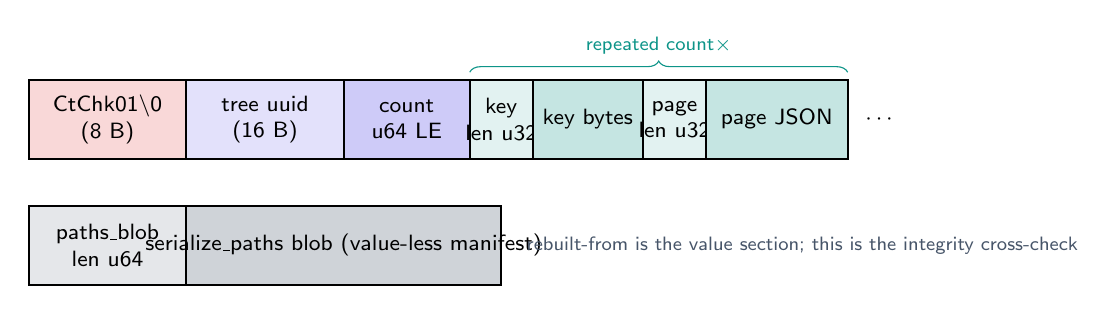
\begin{tikzpicture}[font=\sffamily\footnotesize, x=1cm, y=1cm]
  % header
  \draw[thick, fill=magicc!18] (0,2) rectangle (2.0,3.0); \node[align=center] at (1.0,2.5) {CtChk01\textbackslash0\\(8 B)};
  \draw[thick, fill=metac!16] (2.0,2) rectangle (4.0,3.0); \node[align=center] at (3.0,2.5) {tree uuid\\(16 B)};
  \draw[thick, fill=metac!28] (4.0,2) rectangle (5.6,3.0); \node[align=center] at (4.8,2.5) {count\\u64 LE};
  % repeating frame group
  \draw[thick, fill=framec!12] (5.6,2) rectangle (6.4,3.0); \node[align=center] at (6.0,2.5) {key\\len u32};
  \draw[thick, fill=framec!24] (6.4,2) rectangle (7.8,3.0); \node[align=center] at (7.1,2.5) {key bytes};
  \draw[thick, fill=framec!12] (7.8,2) rectangle (8.6,3.0); \node[align=center] at (8.2,2.5) {page\\len u32};
  \draw[thick, fill=framec!24] (8.6,2) rectangle (10.4,3.0); \node[align=center] at (9.5,2.5) {page JSON};
  % brace over the repeating frame
  \draw[decorate, decoration={brace, amplitude=4pt}, framec] (5.6,3.1) -- (10.4,3.1)
        node[midway, above=3pt, font=\sffamily\scriptsize, framec] {repeated count$\times$};
  \node[anchor=west] at (10.5,2.5) {$\cdots$};
  % trailing paths blob
  \draw[thick, fill=pathc!14] (0,0.4) rectangle (2.0,1.4); \node[align=center] at (1.0,0.9) {paths\_blob\\len u64};
  \draw[thick, fill=pathc!26] (2.0,0.4) rectangle (6.0,1.4); \node[align=center] at (4.0,0.9) {serialize\_paths blob (value-less manifest)};
  \node[anchor=west, font=\sffamily\scriptsize, pathc] at (6.2,0.9) {rebuilt-from is the value section; this is the integrity cross-check};
\end{tikzpicture}
\end{document}
